% python classes slides - basic data types
% (c) 2012 Kostiantyn Danylov aka koder 
% koder.mail@gmail.com
% distributed under CC-BY licence
% http://creativecommons.org/licenses/by/3.0/deed.en

\documentclass{article}
% XeLaTeX
\usepackage{xltxtra}
\usepackage{xunicode}
\usepackage{listings}
\usepackage[landscape]{geometry}

% Fonts
\setmainfont{DejaVu Sans} %{Arial}
\newfontfamily\cyrillicfont{Nimbus Roman No9 L} %{Arial}
\setmonofont{Courier New}
%\setmonofont{Ubuntu Mono}

%\setmonofont{DejaVu Sans Mono}

% Lang
\usepackage{polyglossia}
\setmainlanguage{russian}
\setotherlanguage{english}
\usepackage[dvipsnames,table]{xcolor}


\ifx\pdfoutput\undefined
\usepackage{graphicx}
\else
\usepackage[pdftex]{graphicx}
\fi

\lstset{
	language=python,
	keywordstyle=\color{Emerald},%\texttt, 
	commentstyle=\color{OliveGreen},%\texttt,
	stringstyle=\color{Bittersweet},%\texttt,
	tabsize=4,
	numbers=left,
	xleftmargin=10pt,
	morekeywords={with,as},	
	numberstyle=\large,
	%identifierstyle=\texttt,
	%basicstyle=\texttt,
}

\usepackage{hyperref}

\hypersetup{
	colorlinks=true,
	urlcolor=blue
}

\usepackage{float}
%\floatstyle{boxed} 
%\restylefloat{figure}
\usepackage[normalem]{ulem}


\makeatletter
\def\PY@reset{\let\PY@it=\relax \let\PY@bf=\relax%
    \let\PY@ul=\relax \let\PY@tc=\relax%
    \let\PY@bc=\relax \let\PY@ff=\relax}
\def\PY@tok#1{\csname PY@tok@#1\endcsname}
\def\PY@toks#1+{\ifx\relax#1\empty\else%
    \PY@tok{#1}\expandafter\PY@toks\fi}
\def\PY@do#1{\PY@bc{\PY@tc{\PY@ul{%
    \PY@it{\PY@bf{\PY@ff{#1}}}}}}}
\def\PY#1#2{\PY@reset\PY@toks#1+\relax+\PY@do{#2}}

\expandafter\def\csname PY@tok@gd\endcsname{\def\PY@tc##1{\textcolor[rgb]{0.63,0.00,0.00}{##1}}}
\expandafter\def\csname PY@tok@gu\endcsname{\let\PY@bf=\textbf\def\PY@tc##1{\textcolor[rgb]{0.50,0.00,0.50}{##1}}}
\expandafter\def\csname PY@tok@gt\endcsname{\def\PY@tc##1{\textcolor[rgb]{0.00,0.25,0.82}{##1}}}
\expandafter\def\csname PY@tok@gs\endcsname{\let\PY@bf=\textbf}
\expandafter\def\csname PY@tok@gr\endcsname{\def\PY@tc##1{\textcolor[rgb]{1.00,0.00,0.00}{##1}}}
\expandafter\def\csname PY@tok@cm\endcsname{\let\PY@it=\textit\def\PY@tc##1{\textcolor[rgb]{0.25,0.50,0.50}{##1}}}
\expandafter\def\csname PY@tok@vg\endcsname{\def\PY@tc##1{\textcolor[rgb]{0.10,0.09,0.49}{##1}}}
\expandafter\def\csname PY@tok@m\endcsname{\def\PY@tc##1{\textcolor[rgb]{0.40,0.40,0.40}{##1}}}
\expandafter\def\csname PY@tok@mh\endcsname{\def\PY@tc##1{\textcolor[rgb]{0.40,0.40,0.40}{##1}}}
\expandafter\def\csname PY@tok@go\endcsname{\def\PY@tc##1{\textcolor[rgb]{0.50,0.50,0.50}{##1}}}
\expandafter\def\csname PY@tok@ge\endcsname{\let\PY@it=\textit}
\expandafter\def\csname PY@tok@vc\endcsname{\def\PY@tc##1{\textcolor[rgb]{0.10,0.09,0.49}{##1}}}
\expandafter\def\csname PY@tok@il\endcsname{\def\PY@tc##1{\textcolor[rgb]{0.40,0.40,0.40}{##1}}}
\expandafter\def\csname PY@tok@cs\endcsname{\let\PY@it=\textit\def\PY@tc##1{\textcolor[rgb]{0.25,0.50,0.50}{##1}}}
\expandafter\def\csname PY@tok@cp\endcsname{\def\PY@tc##1{\textcolor[rgb]{0.74,0.48,0.00}{##1}}}
\expandafter\def\csname PY@tok@gi\endcsname{\def\PY@tc##1{\textcolor[rgb]{0.00,0.63,0.00}{##1}}}
\expandafter\def\csname PY@tok@gh\endcsname{\let\PY@bf=\textbf\def\PY@tc##1{\textcolor[rgb]{0.00,0.00,0.50}{##1}}}
\expandafter\def\csname PY@tok@ni\endcsname{\let\PY@bf=\textbf\def\PY@tc##1{\textcolor[rgb]{0.60,0.60,0.60}{##1}}}
\expandafter\def\csname PY@tok@nl\endcsname{\def\PY@tc##1{\textcolor[rgb]{0.63,0.63,0.00}{##1}}}
\expandafter\def\csname PY@tok@nn\endcsname{\let\PY@bf=\textbf\def\PY@tc##1{\textcolor[rgb]{0.00,0.00,1.00}{##1}}}
\expandafter\def\csname PY@tok@no\endcsname{\def\PY@tc##1{\textcolor[rgb]{0.53,0.00,0.00}{##1}}}
\expandafter\def\csname PY@tok@na\endcsname{\def\PY@tc##1{\textcolor[rgb]{0.49,0.56,0.16}{##1}}}
\expandafter\def\csname PY@tok@nb\endcsname{\def\PY@tc##1{\textcolor[rgb]{0.00,0.50,0.00}{##1}}}
\expandafter\def\csname PY@tok@nc\endcsname{\let\PY@bf=\textbf\def\PY@tc##1{\textcolor[rgb]{0.00,0.00,1.00}{##1}}}
\expandafter\def\csname PY@tok@nd\endcsname{\def\PY@tc##1{\textcolor[rgb]{0.67,0.13,1.00}{##1}}}
\expandafter\def\csname PY@tok@ne\endcsname{\let\PY@bf=\textbf\def\PY@tc##1{\textcolor[rgb]{0.82,0.25,0.23}{##1}}}
\expandafter\def\csname PY@tok@nf\endcsname{\def\PY@tc##1{\textcolor[rgb]{0.00,0.00,1.00}{##1}}}
\expandafter\def\csname PY@tok@si\endcsname{\let\PY@bf=\textbf\def\PY@tc##1{\textcolor[rgb]{0.73,0.40,0.53}{##1}}}
\expandafter\def\csname PY@tok@s2\endcsname{\def\PY@tc##1{\textcolor[rgb]{0.73,0.13,0.13}{##1}}}
\expandafter\def\csname PY@tok@vi\endcsname{\def\PY@tc##1{\textcolor[rgb]{0.10,0.09,0.49}{##1}}}
\expandafter\def\csname PY@tok@nt\endcsname{\let\PY@bf=\textbf\def\PY@tc##1{\textcolor[rgb]{0.00,0.50,0.00}{##1}}}
\expandafter\def\csname PY@tok@nv\endcsname{\def\PY@tc##1{\textcolor[rgb]{0.10,0.09,0.49}{##1}}}
\expandafter\def\csname PY@tok@s1\endcsname{\def\PY@tc##1{\textcolor[rgb]{0.73,0.13,0.13}{##1}}}
\expandafter\def\csname PY@tok@sh\endcsname{\def\PY@tc##1{\textcolor[rgb]{0.73,0.13,0.13}{##1}}}
\expandafter\def\csname PY@tok@sc\endcsname{\def\PY@tc##1{\textcolor[rgb]{0.73,0.13,0.13}{##1}}}
\expandafter\def\csname PY@tok@sx\endcsname{\def\PY@tc##1{\textcolor[rgb]{0.00,0.50,0.00}{##1}}}
\expandafter\def\csname PY@tok@bp\endcsname{\def\PY@tc##1{\textcolor[rgb]{0.00,0.50,0.00}{##1}}}
\expandafter\def\csname PY@tok@c1\endcsname{\let\PY@it=\textit\def\PY@tc##1{\textcolor[rgb]{0.25,0.50,0.50}{##1}}}
\expandafter\def\csname PY@tok@kc\endcsname{\let\PY@bf=\textbf\def\PY@tc##1{\textcolor[rgb]{0.00,0.50,0.00}{##1}}}
\expandafter\def\csname PY@tok@c\endcsname{\let\PY@it=\textit\def\PY@tc##1{\textcolor[rgb]{0.25,0.50,0.50}{##1}}}
\expandafter\def\csname PY@tok@mf\endcsname{\def\PY@tc##1{\textcolor[rgb]{0.40,0.40,0.40}{##1}}}
\expandafter\def\csname PY@tok@err\endcsname{\def\PY@bc##1{\setlength{\fboxsep}{0pt}\fcolorbox[rgb]{1.00,0.00,0.00}{1,1,1}{\strut ##1}}}
\expandafter\def\csname PY@tok@kd\endcsname{\let\PY@bf=\textbf\def\PY@tc##1{\textcolor[rgb]{0.00,0.50,0.00}{##1}}}
\expandafter\def\csname PY@tok@ss\endcsname{\def\PY@tc##1{\textcolor[rgb]{0.10,0.09,0.49}{##1}}}
\expandafter\def\csname PY@tok@sr\endcsname{\def\PY@tc##1{\textcolor[rgb]{0.73,0.40,0.53}{##1}}}
\expandafter\def\csname PY@tok@mo\endcsname{\def\PY@tc##1{\textcolor[rgb]{0.40,0.40,0.40}{##1}}}
\expandafter\def\csname PY@tok@kn\endcsname{\let\PY@bf=\textbf\def\PY@tc##1{\textcolor[rgb]{0.00,0.50,0.00}{##1}}}
\expandafter\def\csname PY@tok@mi\endcsname{\def\PY@tc##1{\textcolor[rgb]{0.40,0.40,0.40}{##1}}}
\expandafter\def\csname PY@tok@gp\endcsname{\let\PY@bf=\textbf\def\PY@tc##1{\textcolor[rgb]{0.00,0.00,0.50}{##1}}}
\expandafter\def\csname PY@tok@o\endcsname{\def\PY@tc##1{\textcolor[rgb]{0.40,0.40,0.40}{##1}}}
\expandafter\def\csname PY@tok@kr\endcsname{\let\PY@bf=\textbf\def\PY@tc##1{\textcolor[rgb]{0.00,0.50,0.00}{##1}}}
\expandafter\def\csname PY@tok@s\endcsname{\def\PY@tc##1{\textcolor[rgb]{0.73,0.13,0.13}{##1}}}
\expandafter\def\csname PY@tok@kp\endcsname{\def\PY@tc##1{\textcolor[rgb]{0.00,0.50,0.00}{##1}}}
\expandafter\def\csname PY@tok@w\endcsname{\def\PY@tc##1{\textcolor[rgb]{0.73,0.73,0.73}{##1}}}
\expandafter\def\csname PY@tok@kt\endcsname{\def\PY@tc##1{\textcolor[rgb]{0.69,0.00,0.25}{##1}}}
\expandafter\def\csname PY@tok@ow\endcsname{\let\PY@bf=\textbf\def\PY@tc##1{\textcolor[rgb]{0.67,0.13,1.00}{##1}}}
\expandafter\def\csname PY@tok@sb\endcsname{\def\PY@tc##1{\textcolor[rgb]{0.73,0.13,0.13}{##1}}}
\expandafter\def\csname PY@tok@k\endcsname{\let\PY@bf=\textbf\def\PY@tc##1{\textcolor[rgb]{0.00,0.50,0.00}{##1}}}
\expandafter\def\csname PY@tok@se\endcsname{\let\PY@bf=\textbf\def\PY@tc##1{\textcolor[rgb]{0.73,0.40,0.13}{##1}}}
\expandafter\def\csname PY@tok@sd\endcsname{\let\PY@it=\textit\def\PY@tc##1{\textcolor[rgb]{0.73,0.13,0.13}{##1}}}

\def\PYZbs{\char`\\}
\def\PYZus{\char`\_}
\def\PYZob{\char`\{}
\def\PYZcb{\char`\}}
\def\PYZca{\char`\^}
\def\PYZam{\char`\&}
\def\PYZlt{\char`\<}
\def\PYZgt{\char`\>}
\def\PYZsh{\char`\#}
\def\PYZpc{\char`\%}
\def\PYZdl{\char`\$}
\def\PYZti{\char`\~}
% for compatibility with earlier versions
\def\PYZat{@}
\def\PYZlb{[}
\def\PYZrb{]}
\makeatother

\begin{document}
\LARGE

%-------------------------------------------------------------------------------
\begin{center} Переменные (идентификаторы) \end{center}
\begin{itemize}
	\item Переменные - имена для объектов (ссылки на объект)
	\item Имя - [a-zA-Z\_][a-zA-Z\_0-9]*
	\item Переменная создается присваиванием \\ name = val (a = b = 1 работает, но a = (b = 1) нет)
	\item У одного объекта может быть много имен
	\item Часть имен зарезервирована (for, while, in, ..) \\
			\lstinline!import keyword; print keyword.kwlist!
	\item Типизация динамическая - тип связывается с объектом.
		  Можно считать что все переменные имеют тип (PyObject *)
	\item В компилируемых языков другой подход. Переменная как ящик, 
		  в который кладутся байты и переменная определяет их поведение (тип)
    \item \lstinline!id(obj)! -> int - уникальный идентификатор объекта. Для двух одновременно 
    существующих объектов всегда разный, но может переиспользоваться после уничтожения объекта
\end{itemize}
\newpage

%-------------------------------------------------------------------------------
\begin{center} Переменные \end{center}
\begin{center} 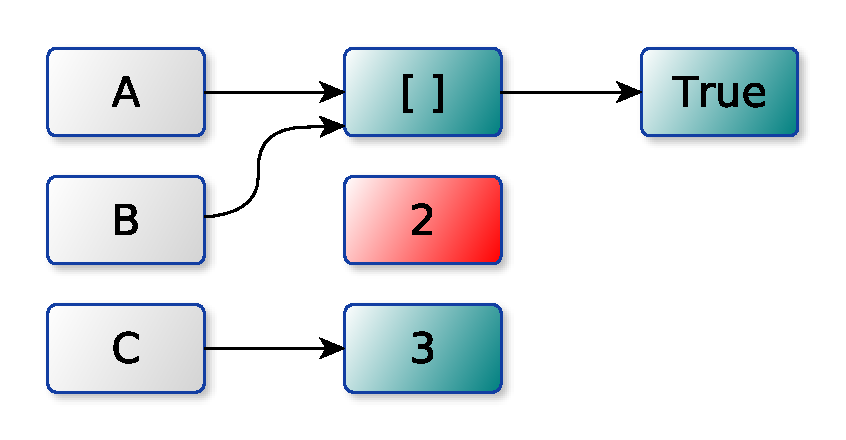
\includegraphics{images/variables.eps} \end{center}
\newpage

%-------------------------------------------------------------------------------
\begin{center} Переменные от 
\href{http://python.net/~goodger/projects/pycon/2007/idiomatic/handout.html}{David Goodger}
\end{center}

\includegraphics{images/a2box.png} \hspace{3cm}

\includegraphics{images/a2tag.png} \hspace{3cm}

\includegraphics{images/ab2tag.png} \\
\newpage

%-------------------------------------------------------------------------------
\begin{center} Переменные \end{center}
Одно и то-же имя(переменная) может в разные моменты указывать на данные разных типов
\vspace{15pt}
\begin{lstlisting}
	x = 12
	x = "12"
\end{lstlisting}
\newpage

%-------------------------------------------------------------------------------
\begin{center} Базовые типы данных \end{center}
\begin{itemize}
	\item None
	\item int
	\item float
	\item str(unicode), byte
	\item bool – True, False
	\item complex - 1 + 2.2j
	\item Elipsis, NotImplemented
\end{itemize}
\newpage

%-------------------------------------------------------------------------------
\begin{center} Базовые типы данных \end{center}
\begin{itemize}
	\item Строгая типизация - не производится автоматических приведений типов, кроме очевидных (int -> float)
	\vspace{15pt}
	\begin{lstlisting}
		1 + "2" # TypeError
		1 + 1.0 == 2.0
		(-1) ** 0.5 # ValueError - no float -> complex conversion
		-1 ** 0.5 == -1 # ??? 
	\end{lstlisting}

	\item Однако все приводится к bool при использовании операций \lstinline|and/or/not| или в 
	        \lstinline|if|
	\begin{lstlisting}
		Empty objects, 0, 0.0, 0 + 0j, None => False
		All else => True
		obj and obj
		obj or obj
	\end{lstlisting}

	\item Типы нужно приводить явно
	\vspace{15pt}
	\begin{lstlisting}
		int("12") == 12
		str(12) == "12"
		repr("12") == "'12'"
		1 + int("2") == 3
	\end{lstlisting}
\end{itemize}
\newpage

%-------------------------------------------------------------------------------
\begin{center} Базовые типы данных \end{center}
Все базовые типы данных - константны. Любая операция создает новый объект.
\begin{lstlisting}
    x = 1
    print id(x) #32230504
    x += 1
    print id(x) #32230480
\end{lstlisting}
\newpage

%-------------------------------------------------------------------------------
\begin{center} Операции с int,  float, complex \end{center}
\begin{itemize}
	\item + - / * \% // **(возведение в степень)
	\item +=, -=, *=, ....
	\item >, <, !=, >=, <=, ==
	\item Не сравнивайте разные типы данных
	\item is vs ==, is not, \lstinline!(a is b) == (id(a) == id(b))!
	\item or and not
	\item \& \hspace{10pt} \textbar \hspace{10pt} \textasciicircum
	\item \lstinline!0 < x == y < 10!
	\item math, cmath
	\item Нет --, ++ (Вместо этого -= 1, += 1 )
\end{itemize}
\newpage

%-------------------------------------------------------------------------------
\begin{center} // vs / \end{center}
\begin{lstlisting}
	3 / 2 == 1.5
	3 / 2.0 == 1.5
	3 // 2 == 1
	3 // 2.0 == 1.0
\end{lstlisting}
\newpage

%-------------------------------------------------------------------------------
\begin{center} Строки \end{center}
\vspace{15pt}
\begin{lstlisting}
	"abc"
	'abc'

	b'abc'
	B'abc'
	b"\xd1\x85\xd0\xb0\xd0\xb9"

	"""abcdef
	gj
	h""" == "abcdef\ngj\nh"

	r"C:\temp\dir\fname" == "C:\\temp\\dir\\fname"

	U"Unicode text"
	RU"Raw unicode text"
\end{lstlisting}
\newpage

%-------------------------------------------------------------------------------
\begin{center} Строковые операции \end{center}
\vspace{15pt}
\begin{lstlisting}
	"abc" > "def" == False
	"abc" + "def" == "abcdef"

	# a * N – a + a + a + … + a, N раз
	"ab" * 3 == "ababab"

	"abcdef"[3] == "d"

	# a[x:y] – substring [x, y)
	"0123456789"[2:4] == "23"

	a.replace(src, dst)
	"x + y".replace("+", "//") == "x // y"

	a.find(string, pos) 
	"abcd".find("cd") => 2
	
	# for x[:x.index(substr)]
	"abcd".find("t") => -1

	"cdabcd".find("cd", 1) => 4

	a.index(string)
	"abc".index("fd") # ValueError

	a.split(string) 
	"a,b,c,d".split(",") == ["a", "b", "c", "d"]

	"abc".startswith("ab") == True
	"abc".endswith("dabc") == False
\end{lstlisting}
\newpage

%-------------------------------------------------------------------------------
\begin{center} Строки форматирование \end{center}
\begin{itemize}
	\item \%, format
\end{itemize}

\vspace{15pt}
\begin{lstlisting}
	"size = %d %s" % (12, 'cm') 
	# "size = 12 cm"

	"size = %(sz)d %(units)s" % dict(sz=1, units='m') 
	# "size = 1 m"

	"Some {} {}".format("very interesting", "text")
	#"Some very interecting text"

	"Brown fox {what} over".format(what="jump")
	#"Brown fox jump over"

	#"{name or index or EMPTY!conversion:format_spec}"
	"{: ^25}".format(xx) == '           xx            '
\end{lstlisting}
\newpage

%-------------------------------------------------------------------------------
%level=3
\begin{center} Unicode \end{center}
\begin{itemize}
	\item Unicode vs encoding
	\item Unicode libraries
	\item Unicode libraries complexity and problems
	\item encode/decode/encoding module
	\item bytes.decode(encoding[, errors]) => string
	\item string.encode(encoding[, errors]) => bytes
	\lstinline!print "\xd1\x85\xd0\xb0\xd0\xb9".decode("utf8")!
	\item Иногда python пытается автоматически перекодировать 
			данные, используя текущую кодировку - sys.getdefaultencoding()
	\item \href{http://www.youtube.com/watch?feature=player_embedded&v=sgHbC6udIqc}
				{Pragmatic Unicode, or, How do I stop the pain?}
\end{itemize}
\newpage

%-------------------------------------------------------------------------------
\begin{center} type \& id \& hash \& isinstance \end{center}
\begin{itemize}
	\item \lstinline!type(x)! => тип x
	\item \lstinline!id(x)! – int идентификатор значения (адрес в памяти)
	\item \lstinline!hash(x)! - int - хэш значения, широко используется внутри питона
	\item \lstinline!isinstance(x, X)! - проверяет, что x имеет тип X.
\end{itemize}
\vspace{15pt}
\begin{lstlisting}
	type(1) == int
	d = "asad"
	type(d) == str
	type(1 is 2) == bool

	id(1) == 34564790 #example
	a is b # same as id(a) == id(b)

	hash(1) == 1
	hash("1") == 1977051568
	isinstance(1, int) == True
	isinstance(1, (str, float)) == False
\end{lstlisting}
\newpage

%-------------------------------------------------------------------------------
%level=3
\begin{center} del \end{center}
\begin{itemize}
	\item Уничтожает переменную(имя), но не объект на который она указывает
	\item Объект будет уничтожен, когда на него никто не будет указывать
\end{itemize}
\begin{lstlisting}
	x = "1"
	y = x
	print(id(x), id(y)) # 139796728292736 139796728292736
	del x
	print(x) # NameError
	print(y, id(y)) # 1 139796728292736
\end{lstlisting}
\newpage

%-------------------------------------------------------------------------------
\end{document}
